\chapter{Lec 21 - Natural Language Processing}

\section{Introduction}
There are over a trillion pages of information on the Web, almost all of it in natural language. An agent that wants to do knowledge acquisition needs to understand (at least partially) the ambiguous, messy languages that humans use. We examine the problem from the point of view of specific information-seeking tasks: text classification, information retrieval, and information extraction. One common factor in addressing these tasks is the use of \textbf{language models}: models that predict the probability distribution of language expressions.

\section{Language models}
Formal languages, such as the programming languages Java or Python, have precisely defined language models. A language can be defined as a set of strings; “print(2 + 2)” is a legal program in the language Python, whereas “2)+(2 print” is not. They are specified by a set of rules called a grammar. Formal languages also have rules that define the meaning or semantics of a program; for example, the rules say that the “meaning” of “2+2” is 4.\\\\
Natural languages, such as English or Spanish, cannot be characterized as a definitive set of sentences. Everyone agrees that “Not to be invited is sad” is a sentence of English, but people disagree on the grammaticality of “To be not invited is sad.” Therefore, it is more fruitful to define a natural language model as a probability distribution over sentences rather than a definitive set.\\\\
Natural languages are also ambiguous. “He saw her duck” can mean either that he saw a waterfowl belonging to her, or that he saw her move to evade something. Thus, again, we cannot speak of a single meaning for a sentence, but rather of a probability distribution over possible meanings.\\\\
Finally, natural languages are difficult to deal with because they are very large, and constantly changing. Thus, our language models are, at best, an approximation.

\section{\textit{N}-gram models}
Ultimately, a written text is composed of characters, letters, digits, punctuation, and spaces in English (and more exotic characters in some other languages). Thus, one of the simplest language models is a probability distribution over sequences of characters. We write $P(c_{1:N})$ for the probability of a sequence of $N$ characters, $c_1$ through $c_N$. A sequence of written symbols of length $n$ is called an $n$-gram. with special case “unigram” for 1-gram, “bigram” for 2-gram, and “trigram” for 3-gram. A model of the probability distribution of $n$-letter sequences is thus called an \textbf{n-gram model}.\\\\
An $n$-gram model is defined as a \textbf{Markov chain} of order $n - 1$.  In a Markov chain the probability of character $c_i$ depends only on the immediately preceding characters, not on any other characters. So in a trigram model (Markov chain of order 2) we have
\[P(c_i | c_{1:i-1}) = P(c_i | c_{i-2:i-1})\]
We can define the probability of a sequence of characters $P(c_{1:N})$ under the trigram model by first factoring with the chain rule and then using the Markov assumption:
\[P(c_{1:N}) = \prod_{i=1}^N P(c_i | c_{1:i-1}) = \prod_{i=1}^N P(c_i | c_{i-2:i-1})\]
For a trigram character model in a language with 100 characters, $\textbf{P}(c_i | c_{i-2:i-1})$ has a million entries ($100^3$), and can be accurately estimated by counting character sequences in a body of text of10 million characters or more. We call a body of text a \textbf{corpus} (plural corpora), from the Latin word for body.\\\\
What can we do with $n$-gram character models? One task for which they are well suited is language identification: given a text, determine what natural language it is written in. One approach to language identification is to first build a trigram character model of each candidate language, $P(c_i | c_{i-2:i-1}, l)$, where the variable $l$ ranges over languages. For each $l$ the model is built by counting trigrams in a corpus of that language  (About 100,000 characters of each language are needed). That gives us a model of $\textbf{P}(Text | Language)$, but we want to select the most probable language given the text, so we apply Bayes’ rule followed by the Markov assumption to get the most probable language:
\[\begin{split}
    l^* & = argmax_l P(l | c_{1:N})\\
    & = argmax_l P(l)P(c_{1:N}|l)\\
    & = argmax_l P(l) \prod_{i=1}^N P(c_i | c_{i-2:i-1}, l)
\end{split}
\]
The trigram model can be learned from a corpus, but what about the prior probability $P(l)$? We may have some estimate of these values; for example, if we are selecting a random Web page we know that English is the most likely language and that the probability of Macedonian will be less than 1\%. The exact number we select for these priors is not critical because the trigram model usually selects one language that is several orders of magnitude more probable than any other.\\\\
Other tasks for character models include spelling correction, genre classification, and named-entity recognition. 

\subsection{Smoothing \textit{n}-gram models}
The major complication of $n$-gram models is that the training corpus provides only an estimate of the true probability distribution. For common character sequences such as "\_th"  any English corpus will give a good estimate.  On the other hand, “\_ht” is very uncommon, no dictionary words start with ht.  It is likely that the sequence would have a count of zero in a training corpus of standard English. Does that mean we should assign $P("ht")=0$?  If we did, then the text “The program issues an http request” would have an English probability of zero, which seems wrong. We have a problem in generalization: we want our language models to generalize well to texts they haven’t seen yet.\\\\
The process od adjusting the probability of low-frequency counts is called \textbf{smoothing}. The simplest type of smoothing was suggested by Pierre-Simon Laplace in the 18th century: he said that, in the lack of further information, if a random Boolean variable $X$ has been false in all $n$ observations so far then the estimate for $P(X = true)$ should be $1/(n+ 2)$. That is, he assumes that with two more trials, one might be true and one false. This technique is called \textbf{Laplace smoothing}.\\\\
A better approach is a \textbf{backoff model}, in which we start by estimating $n$-gram counts, but for any particular sequence that has a low (or zero) count, we back off to $(n - 1)$-grams. \textbf{Linear interpolation} smoothing is a backoff model that combines trigram, bigram, and unigram models by linear interpolation. It defines the probability estimate as
\[\hat{P}(c_i | c_{i-2:i-1}) = \lambda_3 P(c_i | c_{i-2:i-1}) + \lambda_2 P(c_i | c_{i-1}) + \lambda_1 P(c_i)\]
where $\lambda_3 + \lambda_2 + \lambda_1 = 1$.

\section{Model evaluation}
How do we know what model to choose? We can evaluate a model with cross-validation. The evaluation can be a task-specific metric, such as measuring accuracy on language identification, but we would like to define a task-independent language quality model. A different way of describing the probability of a sequence is with a measure called \textbf{perplexity}, defined as
\[Perplexity(c_{1:N}) = P(c_{1:N})^{-\frac{1}{N}}\]
Perplexity can be thought of as the reciprocal of probability, normalized by sequence length. Suppose there are 100 characters in our language, and our model says they are all equally likely. Then for a sequence of any length, the perplexity will be 100.  If some characters are more likely than others, and the model reflects that, then the model will have a perplexity less than 100.

\section{\textit{N}-gram word models}
Now we turn to $n$-gram models over words rather than characters.  All the same mechanism applies equally to word and character models. The main difference is that the \textbf{vocabulary}, the set of symbols that make up the corpus and the model, is larger. There are only about 100 characters in most languages, but with word models we have at least tens of thousands of symbols, and sometimes millions.\\\\
Word $n$-gram models need to deal with \textbf{out of vocabulary} words. With character models, we didn’t have to worry about someone inventing a new letter of the alphabet, but with word models there is always the chance of a new word that was not seen in the training corpus, so we need to model that explicitly in our language model.  This can be done by adding just one new word to the vocabulary: $<UNK>$, standing for the unknown word. We can estimate n-gram counts for $<UNK>$ by this trick:  go through the training corpus, and the first time any individual word appears it is previously unknown, so replace it with the symbol $<UNK>$.  Then compute $n$-gram counts for the corpus as usual, treating $<UNK>$ just like any other word.\\\\
To get a feeling for what word models can do, we built unigram, bigram, and trigram models over the words in this book and then randomly sampled sequences of words from the models. The results are:
\begin{center}
    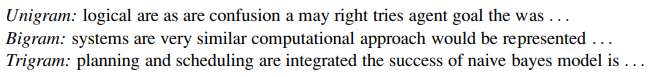
\includegraphics[]{images/n-gram sampling.png}
\end{center}
Even with this small sample, it should be clear that the unigram model is a poor approximation of either English or the content of an AI textbook, and that the bigram and trigram models are much better.

